% =============================================================================
%  COMPUTER VISION -- COMPLETE EXAM PREPARATION NOTES
%  Author:  F. Massaroni
%  Course:  Computer Vision, Prof. Irene Amerini, A.Y. 2024/2025
%  University: Sapienza University of Rome
%              MSc Artificial Intelligence and Robotics
%
%  STRUCTURE
%  ---------
%  PART I   (Ch. 1-11) : Original lecture summary embedded via \includepdf.
%                        The PDF is written in academic English and contains
%                        all course figures; it is included verbatim to
%                        preserve diagrams.
%  ERRATA              : Verified factual corrections to the embedded PDF.
%  PART II  (Ch. 12-18): Advanced topics (Vision Transformers, Diffusion
%                        Models, GANs, GNNs, VLMs, Medical Imaging, MDE,
%                        Efficiency) rewritten in academic English.
%
%  COMPILATION
%  -----------
%  Place  computer_vision.pdf  in the same directory as this file, then:
%      pdflatex computer_vision_final.tex
%      pdflatex computer_vision_final.tex   (twice for correct TOC)
% =============================================================================

\documentclass[12pt,a4paper]{report}

% ---------- encoding / language ----------------------------------------------
\usepackage[utf8]{inputenc}
\usepackage[T1]{fontenc}
\usepackage[english]{babel}

% ---------- mathematics ------------------------------------------------------
\usepackage{amsmath,amsfonts,amssymb,mathtools}
\usepackage{bm}

% ---------- graphics / PDF inclusion ----------------------------------------
\usepackage{graphicx}
\usepackage{pdfpages}   % \includepdf
\usepackage{float}
\usepackage{caption}

% ---------- algorithms -------------------------------------------------------
\usepackage{algorithm}
\usepackage{algpseudocode}

% ---------- tables -----------------------------------------------------------
\usepackage{booktabs}
\usepackage{array}
\usepackage{multirow}

% ---------- lists ------------------------------------------------------------
\usepackage{enumitem}

% ---------- coloured boxes ---------------------------------------------------
\usepackage[most]{tcolorbox}          % [most] required for breakable skins
\tcbuselibrary{breakable,skins}

% ---------- layout -----------------------------------------------------------
\usepackage[top=2.5cm,bottom=2.5cm,left=2.5cm,right=2.5cm,headheight=15pt]{geometry}
\usepackage{fancyhdr}
\usepackage{titlesec}
\usepackage{parskip}
\usepackage{xcolor}

% ---------- hyperlinks (load last) ------------------------------------------
\usepackage[colorlinks=true,
            linkcolor=blue,
            urlcolor=blue,
            citecolor=blue,
            pdftitle={Computer Vision -- Final Exam Notes},
            pdfauthor={F. Massaroni}]{hyperref}

% ---------- coloured box definitions ----------------------------------------
\newtcolorbox{definitionbox}[1][Definition]{
    enhanced, breakable,
    colback=blue!5!white, colframe=blue!65!black,
    fonttitle=\bfseries, title=#1}

\newtcolorbox{importantbox}[1][Important]{
    enhanced, breakable,
    colback=orange!8!white, colframe=orange!75!black,
    fonttitle=\bfseries, title=#1}

\newtcolorbox{formulabox}[1][Key Formula]{
    enhanced, breakable,
    colback=gray!8!white, colframe=gray!60!black,
    fonttitle=\bfseries, title=#1}

\newtcolorbox{examplebox}[1][Example]{
    enhanced, breakable,
    colback=green!5!white, colframe=green!65!black,
    fonttitle=\bfseries, title=#1}

\newtcolorbox{erratabox}[1][Correction]{
    enhanced, breakable,
    colback=red!5!white, colframe=red!65!black,
    fonttitle=\bfseries, title=#1}

\newtcolorbox{warningbox}[1][Warning / Common Pitfall]{
    enhanced, breakable,
    colback=red!4!white, colframe=red!50!black,
    fonttitle=\bfseries, title=#1}

% ---------- header / footer -------------------------------------------------
\pagestyle{fancy}
\fancyhf{}
\fancyhead[L]{\small\textit{Computer Vision -- Exam Notes}}
\fancyhead[R]{\small\textit{\leftmark}}
\fancyfoot[C]{\small\thepage}
\renewcommand{\headrulewidth}{0.4pt}

% ---------- utility commands ------------------------------------------------
\newcommand{\vect}[1]{\mathbf{#1}}
\newcommand{\mat}[1]{\mathbf{#1}}
\newcommand{\norm}[1]{\left\|#1\right\|}

% ============================================================================
\begin{document}
% ============================================================================

% ============================================================================
%  PART I  --  EMBEDDED LECTURE SUMMARY (Chapters 1-11)
% ============================================================================
% The original course summary is already in academic English and contains
% all figures; it is therefore included verbatim rather than re-typeset.

% --- Manual TOC entries so the embedded chapters appear in the index --------
\addcontentsline{toc}{part}{Part I -- Lecture Summary (Ch.~1--11)}
\addcontentsline{toc}{chapter}{1\space\space Image Processing}
\addcontentsline{toc}{chapter}{2.\ Image Pyramids}
\addcontentsline{toc}{chapter}{3.\ Frequency Domain}
\addcontentsline{toc}{chapter}{4.\ Local Features}
\addcontentsline{toc}{chapter}{5.\ Local Descriptors}
\addcontentsline{toc}{chapter}{6.\ Scale-Invariant Feature Transform (SIFT)}
\addcontentsline{toc}{chapter}{7.\ Transformation and Alignment}
\addcontentsline{toc}{chapter}{8.\ Recognition}
\addcontentsline{toc}{chapter}{9.\ Optical Flow}
\addcontentsline{toc}{chapter}{10.\ Camera Calibration}
\addcontentsline{toc}{chapter}{11.\ Epipolar Geometry}

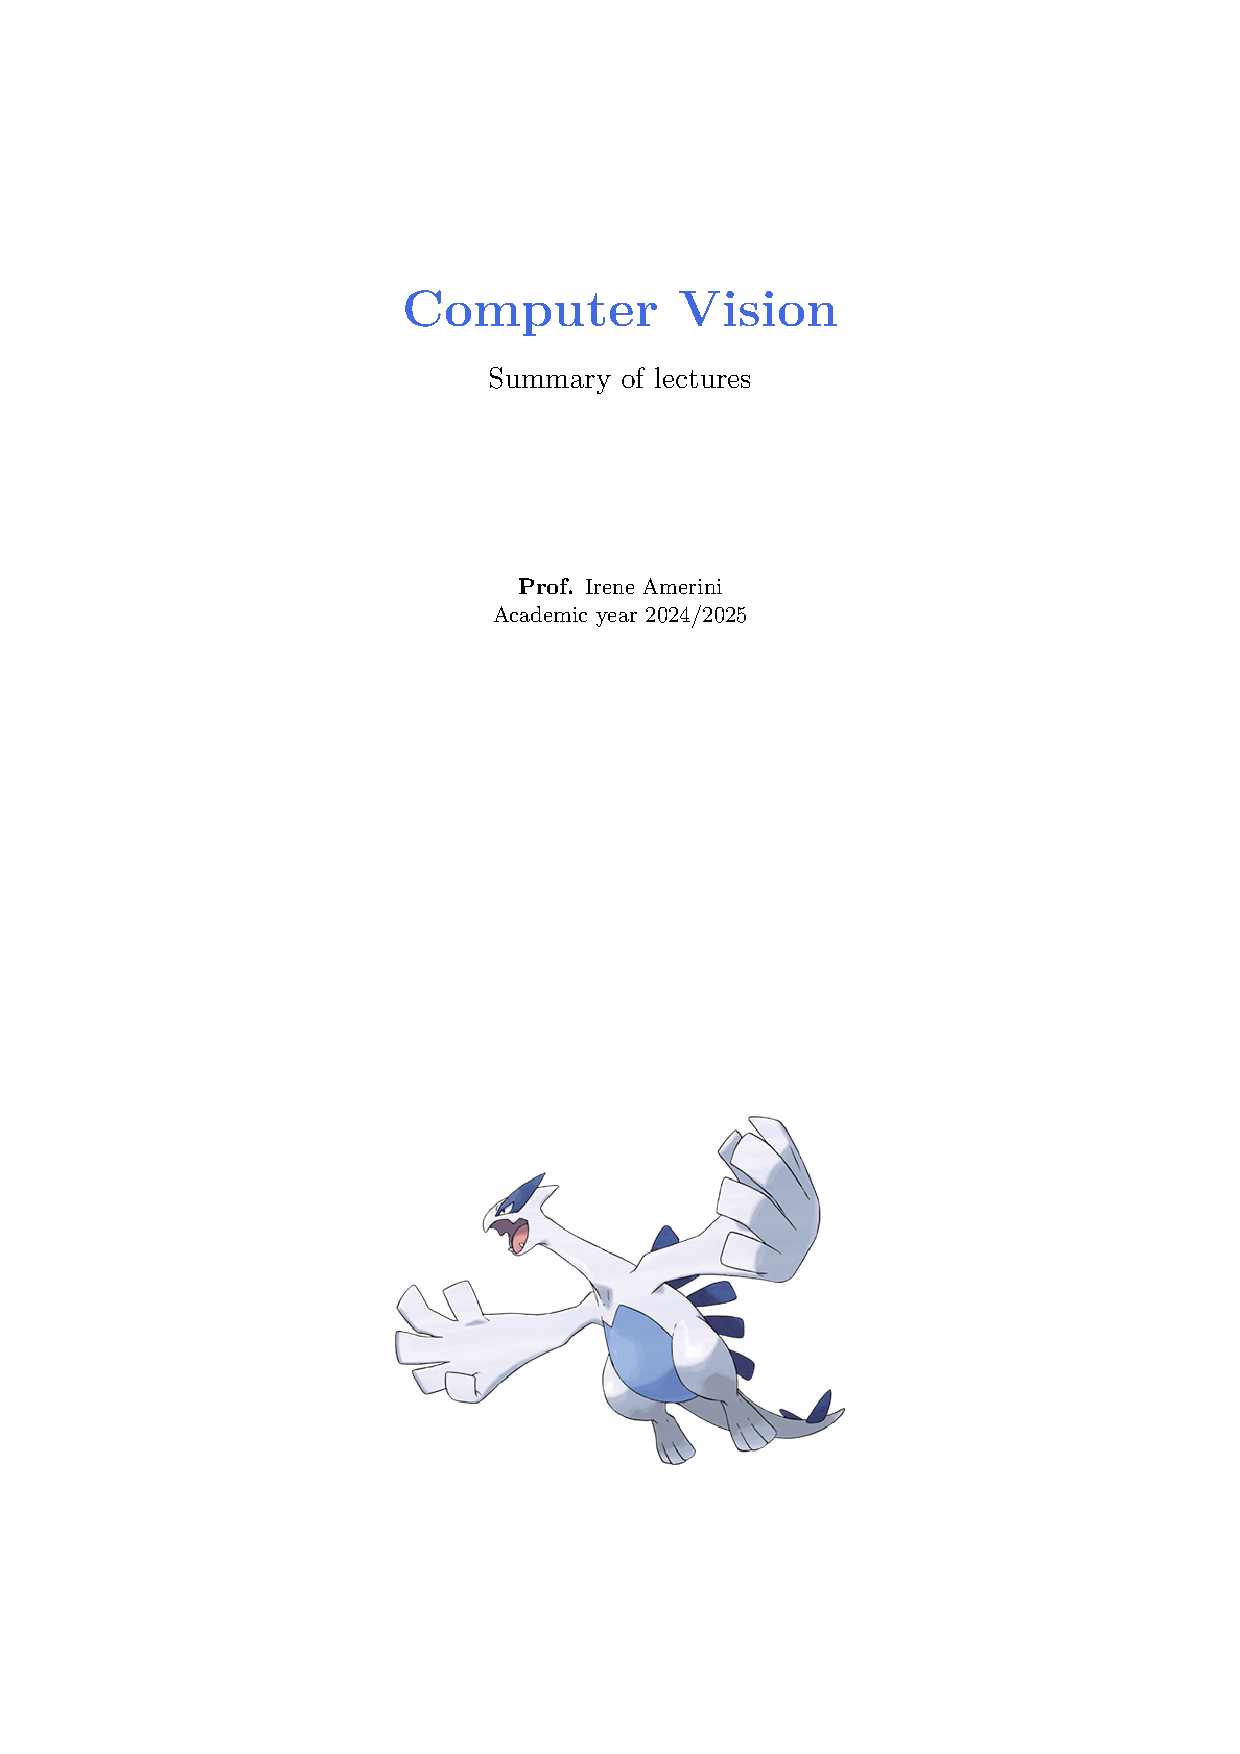
\includepdf[pages=-, fitpaper=true]{computer_vision.pdf}

% ============================================================================
%  ERRATA  --  Corrections to the embedded PDF (Chapters 1-11)
% ============================================================================
\chapter*{Errata and Corrections to Chapters 1--11}
\addcontentsline{toc}{chapter}{Errata and Corrections (Ch.~1--11)}

The embedded PDF is included verbatim and cannot be edited in place.
The following verified factual issues are therefore collected here.

% ---------------------------------------------------------------------------
\section*{E1 \quad Essential matrix: convention inconsistency (\S 11.2--11.3)}

The PDF derivation (pp.~58--59) adopts the pose convention
$\vect{x}' = \vect{R}(\vect{x} - \vect{t})$, which correctly yields
\[
    \vect{E} = \vect{R}\,[\vect{t}]_\times .
\]
However, the same section then writes the fundamental matrix as
$\vect{F} = \vect{K}'^{-T}[\vect{t}]_\times\vect{R}\,\vect{K}^{-1}$,
reversing the factor order $[\vect{t}]_\times \vect{R}$.
This is internally inconsistent with the derivation above.

\begin{erratabox}
Consistent with the PDF's own derivation ($\vect{E} = \vect{R}[\vect{t}]_\times$),
the correct fundamental matrix expression is:
\[
    \vect{F} = \vect{K}'^{-T}\,\vect{E}\,\vect{K}^{-1}
             = \vect{K}'^{-T}\,\vect{R}\,[\vect{t}]_\times\,\vect{K}^{-1}.
\]
\textbf{Exam caveat}: the standard textbook convention (Hartley \& Zisserman)
defines the relative pose as $\vect{x}' = \vect{R}\vect{x} + \vect{t}$,
giving $\vect{E} = [\vect{t}]_\times\vect{R}$.  Both conventions are valid;
always state explicitly which one you adopt.
\end{erratabox}

% ---------------------------------------------------------------------------
\section*{E2 \quad Histogram equalisation: normalisation mismatch (\S 1.1.2)}

The CDF is defined as a normalised cumulative probability,
$\mathrm{CDF}(r_k)=\sum_{i=0}^{k}p(r_i)\in[0,1]$, yet the remapping formula
uses the total pixel count $N$ in the denominator, mixing normalised and
unnormalised quantities.

\begin{erratabox}
Use \emph{cumulative counts} $H(r_k)=\sum_{i=0}^{k}\#\{\text{pixels}=r_i\}$
throughout:
\[
    r_k' = \operatorname{round}\!\left(
        \frac{H(r_k)-H_{\min}}{N-H_{\min}}\,(L-1)
    \right).
\]
Equivalently, with the normalised CDF the denominator is
$1-\mathrm{CDF}_{\min}$:
\[
    r_k' = \operatorname{round}\!\left(
        \frac{\mathrm{CDF}(r_k)-\mathrm{CDF}_{\min}}{1-\mathrm{CDF}_{\min}}\,(L-1)
    \right).
\]
\end{erratabox}

% ---------------------------------------------------------------------------
\section*{E3 \quad SIFT scale sampling: clarification (\S 6.1.1)}

The notes associate $k=\sqrt{2}$ with the scale levels per octave without
explanation.  In Lowe's original formulation the scale multiplier is
$k = 2^{1/s}$, where $s$ is the number of \emph{intervals} per octave.
The default $s=3$ gives $k=2^{1/3}\approx 1.26$; the value $k=\sqrt{2}$
corresponds to $s=2$.  Both choices appear in course material; remember
the general relation $k = 2^{1/s}$.

% ============================================================================
%  PART II  --  ADVANCED TOPICS (Chapters 12-18)
% ============================================================================
\addcontentsline{toc}{part}{Part II -- Advanced Topics (Ch.~12--18)}
\setcounter{chapter}{11}   % continue numbering after Chapter 11

% ============================================================================
\chapter{Vision Transformers}
% ============================================================================

\section{From NLP to Vision: Motivation}

Transformers were introduced in 2017 for natural language processing
[6] and subsequently demonstrated to be highly
effective in computer vision.  The core component is the
\textbf{self-attention} mechanism, which models all pairwise interactions
within an input sequence in a single operation, with no locality bias.

% ---------------------------------------------------------------------------
\section{Self-Attention}

\begin{formulabox}[Scaled Dot-Product Attention]
\[
    \mathrm{Attention}(Q,K,V)
    = \mathrm{softmax}\!\left(\frac{QK^\top}{\sqrt{d_k}}\right)V
\]
\begin{itemize}[itemsep=1pt]
    \item $Q \in \mathbb{R}^{n\times d_k}$: query matrix.
    \item $K \in \mathbb{R}^{m\times d_k}$: key matrix.
    \item $V \in \mathbb{R}^{m\times d_v}$: value matrix.
    \item The scaling $1/\sqrt{d_k}$ prevents the dot products from growing
          large and pushing softmax into regions of near-zero gradient.
\end{itemize}
\end{formulabox}

\subsection{Multi-Head Attention}

\begin{formulabox}[Multi-Head Attention]
\[
    \mathrm{MultiHead}(Q,K,V)
    = \mathrm{Concat}(\mathrm{head}_1,\dots,\mathrm{head}_h)\,W^O
\]
\[
    \mathrm{head}_i
    = \mathrm{Attention}(QW_i^Q,\, KW_i^K,\, VW_i^V)
\]
Each head attends to a different representation subspace; their outputs are
concatenated and linearly projected by $W^O \in \mathbb{R}^{hd_v\times d_\text{model}}$.
\end{formulabox}

\subsection{Positional Encoding}

Self-attention is permutation-equivariant: it has no intrinsic notion of
token order.  A \textbf{positional encoding} is added to the input embeddings
to inject position information.  The original formulation uses fixed sinusoidal
functions; learnable positional embeddings are also common in vision models.

\subsection{Transformer Encoder Block}

Each encoder block applies, in sequence:
\begin{enumerate}[itemsep=1pt]
    \item \textbf{Multi-head self-attention} with residual connection and
          layer normalisation.
    \item \textbf{Feed-forward network} (two linear layers with a non-linearity)
          with residual connection and layer normalisation.
\end{enumerate}

% ---------------------------------------------------------------------------
\section{Vision Transformer (ViT)}

ViT [7] applies a standard Transformer encoder directly
to sequences of image patches.

\subsection{ViT Pipeline}

\begin{enumerate}[itemsep=2pt]
    \item \textbf{Patch extraction}: divide the $H\times W$ image into
          non-overlapping patches of size $P\times P$; this yields
          $N = HW/P^2$ patches.
    \item \textbf{Linear embedding}: flatten each $P\times P\times C$ patch
          into a vector and project to dimension $d_\text{model}$.
    \item \textbf{Prepend class token}: a learnable \texttt{[CLS]} token is
          prepended; its final representation is used for classification.
    \item \textbf{Add positional embeddings} (learnable 1-D encodings).
    \item \textbf{Transformer encoder}: $L$ blocks of multi-head self-attention
          + feed-forward network.
    \item \textbf{Classification head}: MLP applied to the \texttt{[CLS]
          token} output.
\end{enumerate}

\begin{importantbox}[ViT Key Properties]
\begin{itemize}[itemsep=1pt]
    \item Patches act as tokens, analogous to words in NLP.
    \item \textbf{Weak image-specific inductive bias}: unlike CNNs, ViT does
          not build in locality or translation equivariance.  This is an asset
          at very large scale but a liability with limited data.
    \item Highly scalable and parallelisable (all-pairs attention is
          $O(N^2)$ in the number of patches).
    \item Requires large-scale pre-training (ImageNet-21k or JFT-300M) to
          match or outperform CNN baselines.
\end{itemize}
\end{importantbox}

% ---------------------------------------------------------------------------
\section{Swin Transformer}

The Swin Transformer [8] introduces \textbf{shifted-window
attention} to obtain linear complexity and a hierarchical, CNN-like feature
pyramid.

\subsection{Shifted-Window Attention}

Self-attention is computed within local, non-overlapping windows of size
$M\times M$ rather than globally.  Between consecutive layers the windows are
\emph{shifted} by $(\lfloor M/2\rfloor,\lfloor M/2\rfloor)$ pixels, enabling
cross-window connections without increasing cost.

\begin{formulabox}[Complexity Comparison]
\begin{center}
\begin{tabular}{lll}
\toprule
Method & Attention scope & Complexity \\
\midrule
ViT & Global & $O(N^2)$ \\
Swin & Window ($M\!\times\!M$) & $O(N)$ \\
\bottomrule
\end{tabular}
\end{center}
\end{formulabox}

\begin{importantbox}[Swin Advantages]
\begin{itemize}[itemsep=1pt]
    \item Linear complexity $O(N)$ in the number of patches.
    \item Hierarchical, multi-scale representation suitable as a general-purpose
          backbone for detection and segmentation.
    \item Achieved state-of-the-art on COCO detection at the time of its
          introduction (2021).
\end{itemize}
\end{importantbox}

% ---------------------------------------------------------------------------
\section{DETR: End-to-End Object Detection with Transformers}

DETR [9] reformulates object detection as a direct
\emph{set-prediction} problem, eliminating anchors and non-maximum suppression.

\subsection{Architecture}

\begin{enumerate}[itemsep=2pt]
    \item A \textbf{CNN backbone} (e.g.\ ResNet-50) extracts a feature map
          of size $\frac{H}{32}\times\frac{W}{32}\times C$.
    \item A \textbf{Transformer encoder} processes the flattened spatial
          features with positional encodings.
    \item A \textbf{Transformer decoder} takes $N_q$ learnable
          \emph{object queries} and attends to encoder output, producing
          $N_q$ embeddings.
    \item Two \textbf{prediction heads} (MLP and linear) map each embedding
          to a bounding box and a class label (including ``no object'').
    \item A \textbf{bipartite matching loss} (Hungarian algorithm) assigns each
          prediction uniquely to a ground-truth object during training.
\end{enumerate}

\begin{importantbox}[DETR Advantages]
\begin{itemize}[itemsep=1pt]
    \item Fully end-to-end trainable: no hand-crafted anchor boxes, no NMS.
    \item Naturally extends to panoptic segmentation.
    \item Limitation: slow to converge (requires many training epochs); later
          variants (Deformable DETR, DINO) address this.
\end{itemize}
\end{importantbox}

% ---------------------------------------------------------------------------
\section{TimeSformer: Video Recognition}

TimeSformer [16] extends the Transformer to video by
factorising attention over the spatial and temporal dimensions separately
(\emph{divided space-time attention}), which is far cheaper than joint
space-time self-attention.

\begin{enumerate}[itemsep=2pt]
    \item \textbf{Temporal attention}: each patch attends to patches at the
          \emph{same spatial location} across the other frames.
    \item \textbf{Spatial attention}: each patch attends to all other patches
          \emph{within the same frame}.
\end{enumerate}

The two operations are applied sequentially within each Transformer block.

% ============================================================================
\chapter{Generative Adversarial Networks (GANs)}
% ============================================================================

\section{Formulation}

A GAN [11] consists of two networks trained in an
adversarial minimax game:

\begin{itemize}[itemsep=1pt]
    \item \textbf{Generator} $G$: maps a latent vector $z\sim p_z$ to a
          synthetic sample $G(z)$.
    \item \textbf{Discriminator} $D$: outputs the probability that its
          input is a real sample rather than a generated one.
\end{itemize}

\begin{formulabox}[GAN Objective]
\[
    \min_G \max_D\;
    \mathbb{E}_{x\sim p_{\text{data}}}\!\bigl[\log D(x)\bigr]
    + \mathbb{E}_{z\sim p_z}\!\bigl[\log(1 - D(G(z)))\bigr]
\]
At the Nash equilibrium, $G$ recovers $p_{\text{data}}$ and $D \equiv 1/2$.
\end{formulabox}

\section{Training Dynamics and Common Failures}

\begin{itemize}[itemsep=2pt]
    \item \textbf{Mode collapse}: $G$ learns to produce only a few modes of
          the data distribution, ignoring diversity.
    \item \textbf{Vanishing gradients}: when $D$ is too strong, $G$ receives
          near-zero gradients.  The non-saturating loss
          $\max_G\,\mathbb{E}_z[\log D(G(z))]$ alleviates this.
    \item \textbf{Training instability}: the two-player game is inherently
          fragile; careful hyperparameter tuning and architectural choices are
          required.
\end{itemize}

\section{Wasserstein GAN (WGAN)}

WGAN [12] replaces the Jensen--Shannon divergence with the
Wasserstein-1 (Earth Mover's) distance, which provides more stable gradients:

\begin{formulabox}[WGAN Objective]
\[
    \min_G \max_{D \in \mathcal{D}_{1\text{-Lip}}}
    \mathbb{E}_{x\sim p_{\text{data}}}[D(x)]
    - \mathbb{E}_{z\sim p_z}[D(G(z))]
\]
$D$ is constrained to the class of 1-Lipschitz functions (enforced by weight
clipping or gradient penalty in WGAN-GP).
\end{formulabox}

\section{Notable Architectures}

\begin{itemize}[itemsep=2pt]
    \item \textbf{DCGAN}: deep convolutional GAN; uses batch normalisation,
          strided convolutions, and ReLU/LeakyReLU — the canonical baseline.
    \item \textbf{Conditional GAN (cGAN)}: conditions both $G$ and $D$ on a
          class label or input image, enabling class-conditional generation.
    \item \textbf{CycleGAN}: unsupervised image-to-image translation using
          two generators and a \emph{cycle-consistency loss}
          ($G(F(x)) \approx x$) to enforce bijective mapping without paired
          training data.
    \item \textbf{StyleGAN}: disentangles high-level attributes (style) from
          stochastic details (noise) via adaptive instance normalisation (AdaIN)
          applied at each resolution level; produces photorealistic faces.
    \item \textbf{BigGAN}: large-scale conditional GAN, achieving high
          FID/IS scores on ImageNet at $512\times512$.
\end{itemize}

\section{Evaluation Metrics}

\begin{itemize}[itemsep=2pt]
    \item \textbf{Inception Score (IS)}: measures quality (high
          $p(y|x)$) and diversity (high $p(y)$ entropy) jointly.  Higher
          is better; does not compare to real data distribution.
    \item \textbf{Fréchet Inception Distance (FID)}: measures the Fréchet
          distance between real and generated feature distributions (from
          Inception-v3):
          \[
              \mathrm{FID} = \|\mu_r - \mu_g\|^2
              + \mathrm{tr}\!\bigl(\Sigma_r + \Sigma_g
              - 2(\Sigma_r\Sigma_g)^{1/2}\bigr)
          \]
          Lower is better; sensitive to mode collapse and mode dropping.
\end{itemize}

% ============================================================================
\chapter{Diffusion Models}
% ============================================================================

\section{Overview of Deep Generative Models}

\begin{center}
\begin{tabular}{llll}
\toprule
Model & Training & Sampling & Strengths \\
\midrule
VAE    & ELBO               & single pass (fast) & stable, disentangled \\
GAN    & adversarial        & single pass (fast) & sharp images \\
Flow   & exact likelihood   & single pass        & exact density \\
Diffusion & denoising score & iterative (slow)   & best quality, diversity \\
\bottomrule
\end{tabular}
\end{center}

\section{DDPM: Denoising Diffusion Probabilistic Models}

A diffusion model [10] defines a fixed \emph{forward} process
that gradually corrupts a real image with Gaussian noise until only pure noise
remains, and learns a parametric \emph{reverse} process that iteratively
denoises, generating images from noise.

\subsection{Forward Process}

\begin{formulabox}[Forward (Noising) Process]
\[
    q(x_t \mid x_{t-1})
    = \mathcal{N}\!\bigl(x_t;\;\sqrt{1-\beta_t}\,x_{t-1},\;\beta_t\mat{I}\bigr),
    \qquad t = 1,\dots,T
\]
where $\{\beta_t\}$ is a fixed variance schedule ($0 < \beta_t < 1$,
monotonically increasing).
\end{formulabox}

Defining $\alpha_t = 1-\beta_t$ and
$\bar\alpha_t = \prod_{i=1}^{t}\alpha_i$, the reparameterisation trick
gives a closed-form expression for any $t$:

\begin{formulabox}[Reparameterisation (Key Identity)]
\[
    x_t = \sqrt{\bar\alpha_t}\,x_0 + \sqrt{1-\bar\alpha_t}\,\epsilon,
    \qquad \epsilon \sim \mathcal{N}(0,\mat{I})
\]
This allows sampling $x_t$ at \emph{any} timestep directly from $x_0$,
without iterating through $t$ steps.
\end{formulabox}

\subsection{Reverse Process}

A neural network $\epsilon_\theta$ (typically a U-Net) parameterises the
reverse (denoising) transitions:
\[
    p_\theta(x_{t-1}\mid x_t)
    = \mathcal{N}\!\bigl(x_{t-1};\;\mu_\theta(x_t,t),\;\Sigma_\theta(x_t,t)\bigr).
\]

\subsection{Training Objective}

After deriving a variational lower bound (ELBO) and simplifying, the
training objective reduces to a \textbf{noise-prediction} (denoising) loss:

\begin{formulabox}[DDPM Training Loss]
\[
    L_{\text{simple}}
    = \mathbb{E}_{x_0,\,\epsilon,\,t}
      \Bigl[\,\bigl\|\epsilon - \epsilon_\theta(x_t,t)\bigr\|^2\,\Bigr]
\]
The network learns to predict the noise $\epsilon$ that was added to produce
$x_t$.
\end{formulabox}

\subsection{Training and Sampling Algorithms}

\begin{algorithm}[H]
\caption{DDPM Training}
\begin{algorithmic}[1]
\Repeat
    \State Sample $x_0 \sim q(x_0)$
    \State Sample $t \sim \mathrm{Uniform}(\{1,\dots,T\})$
    \State Sample $\epsilon \sim \mathcal{N}(0,\mat{I})$
    \State Compute $x_t \gets \sqrt{\bar\alpha_t}\,x_0 + \sqrt{1-\bar\alpha_t}\,\epsilon$
    \State Take gradient step on $\nabla_\theta\,\|\epsilon - \epsilon_\theta(x_t,t)\|^2$
\Until{converged}
\end{algorithmic}
\end{algorithm}

\begin{algorithm}[H]
\caption{DDPM Sampling}
\begin{algorithmic}[1]
\State Sample $x_T \sim \mathcal{N}(0,\mat{I})$
\For{$t = T, T-1, \dots, 1$}
    \State $z \gets \mathcal{N}(0,\mat{I})$ if $t > 1$, else $z \gets 0$
    \State $\displaystyle x_{t-1} \gets \frac{1}{\sqrt{\alpha_t}}\!\left(x_t - \frac{\beta_t}{\sqrt{1-\bar\alpha_t}}\,\epsilon_\theta(x_t,t)\right) + \sigma_t z$
\EndFor
\State \Return $x_0$
\end{algorithmic}
\end{algorithm}

\begin{importantbox}[Diffusion vs.\ GAN]
\begin{itemize}[itemsep=1pt]
    \item Diffusion models produce \textbf{higher diversity} and avoid mode
          collapse; training is \textbf{stable} (no adversarial game).
    \item Disadvantage: \textbf{slow sampling} ($T = 1000$ steps by default);
          mitigated by DDIM (deterministic sampling, $\sim$50 steps) and
          consistency models (1--2 steps).
\end{itemize}
\end{importantbox}

\section{Applications}

Image generation (DALL·E~2, Stable Diffusion, Midjourney), video generation
(Sora), text-to-image translation, image inpainting, super-resolution,
and medical image synthesis.

% ============================================================================
\chapter{Graph Neural Networks (GNNs)}
% ============================================================================

\section{Graphs and Their Representations}

A graph $G=(V,E)$ consists of a node set $V$ ($|V|=n$) and an edge set $E$.
Node features are collected in a matrix $\mat{H}\in\mathbb{R}^{n\times d}$.

\begin{itemize}[itemsep=2pt]
    \item \textbf{Adjacency matrix} $\mat{A}\in\{0,1\}^{n\times n}$: dense,
          $O(n^2)$ storage.
    \item \textbf{Adjacency list}: sparse representation, $O(n+|E|)$ storage.
    \item \textbf{Degree matrix} $\mat{D}$: diagonal, $D_{ii}=\sum_j A_{ij}$.
\end{itemize}

\textbf{Key structural properties}:
\begin{itemize}[itemsep=1pt]
    \item \textbf{Variable size}: the number of nodes and edges varies.
    \item \textbf{Non-Euclidean domain}: no intrinsic spatial coordinates.
    \item \textbf{Permutation invariance}: graph-level tasks must be invariant
          to node reordering.
\end{itemize}

\section{Message Passing}

Message passing is the core computational paradigm of GNNs.  Node
representations are iteratively updated by aggregating information from
neighbours:

\begin{formulabox}[General Message Passing]
\[
    h_u^{(k+1)} = \mathrm{UPDATE}^{(k)}\!\Bigl(h_u^{(k)},\;
    \mathrm{AGGREGATE}^{(k)}\!\bigl(\{\,h_v^{(k)} : v\in\mathcal{N}(u)\,\}\bigr)\Bigr)
\]
$\mathrm{AGGREGATE}$ must be \textbf{permutation-invariant}
(e.g.\ $\sum$, mean, max).
\end{formulabox}

\section{GNN Variants}

\subsection{Graph Convolutional Network (GCN)}

\begin{formulabox}[GCN Layer]
\[
    \mat{H}^{(l+1)}
    = \sigma\!\Bigl(\tilde{\mat{D}}^{-\frac12}\,\tilde{\mat{A}}\,
      \tilde{\mat{D}}^{-\frac12}\,\mat{H}^{(l)}\,\mat{W}^{(l)}\Bigr)
\]
$\tilde{\mat{A}} = \mat{A} + \mat{I}$ adds self-loops;
$\tilde{\mat{D}}$ is the degree matrix of $\tilde{\mat{A}}$.
\end{formulabox}

Symmetric normalisation $\tilde{\mat{D}}^{-1/2}\tilde{\mat{A}}\tilde{\mat{D}}^{-1/2}$
prevents feature magnitude from growing with node degree.

\subsection{Graph Attention Network (GAT)}

GATs replace the fixed normalisation weights with \emph{learned} attention
coefficients:

\begin{formulabox}[GAT Attention]
\[
    e_{ij} = \mathrm{LeakyReLU}\!\bigl(\vect{a}^\top[\mat{W}h_i \,\|\, \mat{W}h_j]\bigr),
    \qquad
    \alpha_{ij} = \frac{\exp(e_{ij})}{\sum_{k\in\mathcal{N}_i}\exp(e_{ik})}
\]
\[
    h_i' = \Big\|_{k=1}^{K}\,\sigma\!\!\left(\sum_{j\in\mathcal{N}_i}\alpha_{ij}^{k}\mat{W}^{k}h_j\right)
\]
where $\|$ denotes concatenation over $K$ attention heads.
\end{formulabox}

\subsection{Limitations}

\begin{itemize}[itemsep=1pt]
    \item \textbf{Over-smoothing}: with many layers, node features converge to
          indistinguishable values.
    \item \textbf{Structural sensitivity}: performance depends on graph quality.
    \item \textbf{Scalability}: full neighbourhood aggregation is expensive for
          large graphs; mini-batch sampling methods (GraphSAGE, ClusterGCN) are
          used in practice.
\end{itemize}

% ============================================================================
\chapter{Vision-Language Models (VLMs)}
% ============================================================================

\section{Motivation}

Unimodal models are fundamentally limited: vision models extract spatial
features but lack semantic reasoning, whereas language models handle syntax
and context but lack perceptual grounding.  Multimodal models jointly
represent both modalities, enabling tasks such as visual question answering,
image captioning, and zero-shot recognition.

\section{Fusion Strategies}

\begin{center}
\begin{tabular}{lll}
\toprule
Strategy & Modalities fused at & Example \\
\midrule
Early fusion  & Input level       & Single shared Transformer \\
Intermediate  & Mid-network       & Flamingo (gated cross-attention) \\
Late fusion   & Output/prediction & Ensemble of unimodal models \\
\bottomrule
\end{tabular}
\end{center}

\section{CLIP: Contrastive Language-Image Pre-Training}

CLIP [15] is trained on $\sim$400 million web-scraped
image-text pairs using \textbf{contrastive learning}.

\subsection{Architecture}

\begin{itemize}[itemsep=1pt]
    \item \textbf{Image encoder}: ViT or ResNet; maps images to
          $\ell_2$-normalised embeddings $\vect{I}_k$.
    \item \textbf{Text encoder}: Transformer; maps tokenised captions to
          $\ell_2$-normalised embeddings $\vect{T}_k$.
    \item Training maximises the cosine similarity of matching pairs and
          minimises it for non-matching pairs within a batch.
\end{itemize}

\subsection{InfoNCE Loss}

For a batch of $N$ image-text pairs with temperature $\tau$:

\begin{formulabox}[CLIP InfoNCE Loss]
\[
    \mathcal{L}_{I\to T}
    = -\sum_{k=1}^{N}\log
      \frac{\exp(\vect{I}_k\!\cdot\vect{T}_k/\tau)}
           {\sum_{j=1}^{N}\exp(\vect{I}_k\!\cdot\vect{T}_j/\tau)},
    \quad
    \mathcal{L}_{T\to I}
    = -\sum_{k=1}^{N}\log
      \frac{\exp(\vect{I}_k\!\cdot\vect{T}_k/\tau)}
           {\sum_{j=1}^{N}\exp(\vect{I}_j\!\cdot\vect{T}_k/\tau)}
\]
\[
    \mathcal{L}_{\text{CLIP}} = \tfrac{1}{2}\bigl(\mathcal{L}_{I\to T}
    + \mathcal{L}_{T\to I}\bigr)
\]
The loss forms an $N\times N$ similarity matrix; the diagonal is the set of
positive pairs.
\end{formulabox}

\subsection{Zero-Shot Transfer}

At inference, class names are embedded as text prompts
(e.g.\ ``a photo of a \{class\}''); the image is classified by finding the
most similar text embedding.  No task-specific fine-tuning is required.

\begin{importantbox}[Why CLIP Works]
\begin{itemize}[itemsep=1pt]
    \item \textbf{Zero annotation cost}: supervision comes from naturally
          occurring image-text pairs scraped from the web.
    \item \textbf{Scale}: hundreds of millions of pairs.
    \item \textbf{Strong zero-shot transfer}: flexible via prompt engineering.
    \item \textbf{Limitations}: no generative capability; limited counting
          and reasoning; sensitive to prompt design.
\end{itemize}
\end{importantbox}

\section{Modern VLMs}

\begin{itemize}[itemsep=2pt]
    \item \textbf{BLIP}: unifies understanding (contrastive + matching) and
          generation (language modelling) in a single pre-training framework.
    \item \textbf{Flamingo}: uses a frozen vision encoder and a frozen LLM
          connected by a Perceiver Resampler and gated cross-attention layers;
          strong few-shot learner.
    \item \textbf{Instruction tuning}: supervised fine-tuning on
          (system prompt, instruction + image, gold response) triples to
          improve instruction-following.
    \item \textbf{In-context learning (ICL)}: few-shot prompting without
          updating model weights.
    \item \textbf{Chain-of-thought (CoT)}: the model generates intermediate
          reasoning steps before the final answer, reducing hallucination.
\end{itemize}

% ============================================================================
\chapter{Medical Imaging}
% ============================================================================

\section{Imaging Modalities}

\begin{itemize}[itemsep=2pt]
    \item \textbf{X-ray}: electromagnetic radiation; high contrast for bone
          and lung pathology; dense tissue appears white, air appears black.
          Low cost, fast acquisition; 2-D projection.
    \item \textbf{CT (Computed Tomography)}: ionising radiation;
          3-D reconstruction from many X-ray projections at different angles.
          Used for trauma, tumours, and vascular disease.
    \item \textbf{MRI (Magnetic Resonance Imaging)}: strong magnetic fields
          + radiofrequency pulses; best soft-tissue contrast (brain, abdomen);
          no ionising radiation; slow acquisition; sensitive to motion.
    \item \textbf{Ultrasound}: high-frequency sound waves; real-time imaging
          of organs, muscles, and foetuses; portable, low cost; operator-
          dependent, noisy (speckle).
    \item \textbf{PET (Positron Emission Tomography)}: functional imaging of
          metabolic activity (e.g.\ tumour staging); low spatial resolution;
          commonly fused with CT (PET-CT).
\end{itemize}

\section{The Medical Data Gap}

\begin{itemize}[itemsep=1pt]
    \item \textbf{Volume}: medical datasets are orders of magnitude smaller
          than ImageNet.
    \item \textbf{Annotation}: requires expert knowledge (radiologists,
          pathologists); expensive and time-consuming.
    \item \textbf{Privacy}: strict regulation (GDPR, HIPAA) limits data
          sharing.
    \item \textbf{Domain characteristics}: low contrast, imaging artefacts,
          significant inter-scanner and inter-site variability.
    \item \textbf{Consequence}: models trained on one centre/scanner generalise
          poorly to others (\emph{domain shift}).
\end{itemize}

\textbf{Mitigation strategies}: transfer learning from ImageNet or
natural-image pre-trained models, data augmentation, federated learning,
self-supervised pre-training, and meta-learning.

\section{Segmentation Architectures}

\begin{itemize}[itemsep=2pt]
    \item \textbf{U-Net}: encoder--decoder with \emph{skip connections} that
          pass feature maps from the encoder directly to the decoder, combining
          high-level semantics with fine-grained spatial detail.
          De facto standard for biomedical segmentation.
    \item \textbf{U-Net++}: nested skip connections providing multiple fusion
          paths at each scale.
    \item \textbf{TransUNet}: U-Net with a ViT encoder (applied at the
          bottleneck); captures long-range context at higher computational cost.
    \item \textbf{3D segmentation}: processes the full volumetric stack
          (CT/MRI volumes); captures inter-slice context and ensures
          3-D consistency; greatly increases memory and training cost.
\end{itemize}

\section{Loss Functions}

\begin{formulabox}[Dice Loss (class-imbalance robust)]
\[
    L_{\text{dice}} = 1 - \frac{1}{C}\sum_{c=0}^{C-1}
    \frac{2\sum_{n=1}^{N} t_n^c\,y_n^c}
         {\sum_{n=1}^{N}\bigl(t_n^c + y_n^c\bigr)}
\]
Directly optimises the overlap between prediction and ground truth;
insensitive to class frequency.
\end{formulabox}

\begin{formulabox}[Focal Loss (hard-example mining)]
\[
    L_{\text{focal}}
    = -\sum_{n=1}^{N}(1 - p_{t,n})^{\gamma}\,\log p_{t,n},
    \qquad p_{t,n} = t_n \cdot y_n
\]
Down-weights well-classified (easy) examples, focusing training on hard
cases such as small lesions.  Typically $\gamma = 2$.
\end{formulabox}

In practice, the \textbf{combined Dice + Cross-Entropy loss} is commonly used:
$L = L_{\text{dice}} + L_{\text{CE}}$.

\section{Evaluation Metrics}

\textbf{Detection}: IoU, Average Precision (AP), mean AP (mAP) at various
IoU thresholds.

\textbf{Segmentation}:

\begin{itemize}[itemsep=1pt]
    \item \textbf{Dice score} (DSC): $\frac{2|X\cap Y|}{|X|+|Y|}$
          — equivalent to the F1 score; measures overlap.
    \item \textbf{Hausdorff Distance (HD)}:
          \[
              \mathrm{HD}(X,Y)
              = \max\!\Bigl(\max_{x\in X}\min_{y\in Y}\|x-y\|,\;
                            \max_{y\in Y}\min_{x\in X}\|x-y\|\Bigr)
          \]
          Measures the worst-case surface-to-surface deviation; sensitive to
          outliers (the 95th-percentile HD is often preferred).
\end{itemize}

\section{Foundation Models for Medical Imaging}

\begin{itemize}[itemsep=2pt]
    \item \textbf{MedSAM / MedSAM2}: Segment Anything Model adapted to medical
          imaging; enables prompted 3-D segmentation from 2-D interactive
          inputs; reduces manual annotation burden by $>85\%$.
    \item \textbf{UniMed-CLIP}: a unified VLM trained on 5.3M image-text pairs
          across six medical modalities (X-ray, CT, MRI, etc.); open-source.
    \item \textbf{UniChest}: federated multi-hospital training with
          shared global knowledge plus hospital-specific expert modules.
\end{itemize}

% ============================================================================
\chapter{Monocular Depth Estimation (MDE)}
% ============================================================================

\section{Problem Statement}

Depth information is lost when a 3-D scene is projected onto a 2-D image.
Recovering depth from a \emph{single} image is therefore an inherently
ill-posed problem: infinitely many 3-D scenes can produce the same 2-D
image.  The task is nevertheless tractable because images contain rich
monocular cues.

\subsection{Monocular Cues}

\begin{itemize}[itemsep=1pt]
    \item Linear perspective (converging parallel lines).
    \item Relative size (known objects appear smaller at greater depth).
    \item Texture gradient (texture elements become smaller with distance).
    \item Occlusion (near objects overlap far objects).
    \item Atmospheric haze (distant objects appear less saturated).
\end{itemize}

\section{Learning Approaches}

\begin{itemize}[itemsep=2pt]
    \item \textbf{Fully supervised}: requires dense ground-truth depth maps
          (from LiDAR or structured light); best accuracy.
    \item \textbf{Semi-supervised}: uses sparse depth (e.g.\ LiDAR) combined
          with image reconstruction consistency.
    \item \textbf{Self-supervised / Unsupervised}: minimises photometric
          reprojection error between video frames or stereo pairs; no depth
          labels required; accuracy lower than supervised methods.
\end{itemize}

\section{Evaluation Metrics}

\textbf{Error metrics (lower is better)}:
\begin{itemize}[itemsep=1pt]
    \item Absolute Relative Error (AbsRel):
          $\frac{1}{|P|}\sum_i |p_i-g_i|/g_i$
    \item Root Mean Squared Error (RMSE):
          $\sqrt{\frac{1}{|P|}\sum_i(p_i-g_i)^2}$
    \item $\log_{10}$ error: $\frac{1}{|P|}\sum_i|\log_{10}p_i-\log_{10}g_i|$
\end{itemize}

\begin{formulabox}[Threshold Accuracy $\delta_i$ (higher is better)]
\[
    \delta_i = \frac{1}{|P|}\,\Bigl|\Bigl\{p_i \;:\;
    \max\!\Bigl(\tfrac{p_i}{g_i},\,\tfrac{g_i}{p_i}\Bigr)
    < 1.25^i \Bigr\}\Bigr|, \quad i \in \{1,2,3\}
\]
The fraction of predicted depths $p_i$ that agree with the ground truth $g_i$
within a factor of $1.25^i$.
\end{formulabox}

\section{Depth Anything v2}

Depth Anything v2 follows a \textbf{synthetic-to-real pseudo-labelling}
pipeline:
\begin{enumerate}[itemsep=1pt]
    \item Train a \emph{teacher} model on synthetic data (perfect ground truth,
          no domain-adaptation noise).
    \item Generate pseudo-labels on a large set of real unlabelled images
          using the teacher.
    \item Train a \emph{student} model on the pseudo-labelled real data,
          achieving strong real-world generalisation.
\end{enumerate}

\section{Application: RGB-D for Deepfake Detection}

Combining an RGB image with a depth map estimated by MDE exposes geometric
inconsistencies introduced by face manipulation (blending boundaries,
unnatural 3-D structure), improving deepfake detection accuracy compared to
RGB-only approaches.

% ============================================================================
\chapter{Efficiency in Deep Learning}
% ============================================================================

\section{Efficient Training vs.\ Efficient Inference}

\begin{itemize}[itemsep=2pt]
    \item \textbf{Efficient training}: reduce wall-clock training time and
          optimise GPU/TPU utilisation (mixed-precision training, gradient
          checkpointing, distributed data parallelism).
    \item \textbf{Efficient inference}: minimise latency and resource
          consumption when deploying a trained model on new data
          (particularly relevant for edge/mobile deployment).
\end{itemize}

\section{Techniques for Efficient Inference}

\begin{itemize}[itemsep=2pt]
    \item \textbf{Compact architectures}: design models with lower intrinsic
          complexity (e.g.\ linear-attention variants, MobileNet depthwise
          separable convolutions, EfficientNet compound scaling).
    \item \textbf{Pruning}: remove parameters (neurons, filters, or
          connections) that contribute least to task performance, based on
          magnitude or gradient-based importance scores.
    \item \textbf{Knowledge distillation}: train a small \emph{student} to
          mimic the outputs (soft logits, intermediate features) of a large
          pre-trained \emph{teacher}.
    \item \textbf{Quantisation}: reduce numerical precision of weights and
          activations (e.g.\ FP32 $\to$ INT8 or INT4), decreasing memory
          footprint and enabling integer arithmetic on hardware accelerators.
    \item \textbf{Structured vs.\ unstructured pruning}: structured pruning
          (removing whole filters/heads) yields hardware-friendly speedup;
          unstructured pruning (individual weights) achieves higher sparsity
          but requires sparse hardware support.
\end{itemize}

\section{Efficiency Metrics}

\begin{itemize}[itemsep=1pt]
    \item \textbf{MACs}: multiply-accumulate operations — primary measure of
          model computational cost.
    \item \textbf{FLOPs}: floating-point operations ($\approx 2\times$ MACs).
    \item \textbf{Parameter count}: memory footprint of the model weights.
    \item \textbf{Latency}: wall-clock inference time on target hardware.
    \item \textbf{Throughput}: images processed per second.
\end{itemize}

\section{Efficiency--Performance Trade-off}

\begin{itemize}[itemsep=2pt]
    \item \textbf{Pareto frontier}: the set of model configurations for which
          no other configuration is both more efficient \emph{and} more
          accurate.
    \item \textbf{Efficiency Error Rate (EER)}: a composite metric that
          aggregates efficiency measures relative to a reference model $R$:
          \[
              \mathrm{EER} = \frac{1}{|I|}\sum_{i\in I}\frac{M_i}{R_i}
          \]
          where $M_i$ is the value of metric $i$ for the candidate model and
          $R_i$ for the reference.
\end{itemize}

% ============================================================================
%  REFERENCES
% ============================================================================
\chapter*{References}
\addcontentsline{toc}{chapter}{References}

\begin{enumerate}[itemsep=2pt, label={[\arabic*]}]
    \item Szeliski, R. (2022). \textit{Computer Vision: Algorithms and
          Applications}, 2nd ed. Springer.
    \item Hartley, R., \& Zisserman, A. (2004). \textit{Multiple View
          Geometry in Computer Vision}, 2nd ed. Cambridge University Press.
    \item Forsyth, D.~A., \& Ponce, J. (2011). \textit{Computer Vision:
          A Modern Approach}, 2nd ed. Pearson.
    \item Goodfellow, I., Bengio, Y., \& Courville, A. (2016).
          \textit{Deep Learning}. MIT Press.
    \item \label{lowe2004} Lowe, D.~G. (2004). Distinctive Image Features
          from Scale-Invariant Keypoints. \textit{IJCV}, 60(2), 91--110.
    \item \label{vaswani2017attention} Vaswani, A., et al. (2017). Attention
          Is All You Need. \textit{NeurIPS}.
    \item \label{dosovitskiy2021vit} Dosovitskiy, A., et al. (2021). An
          Image is Worth $16\!\times\!16$ Words: Transformers for Image
          Recognition at Scale. \textit{ICLR}.
    \item \label{liu2021swin} Liu, Z., et al. (2021). Swin Transformer:
          Hierarchical Vision Transformer Using Shifted Windows. \textit{ICCV}.
    \item \label{carion2020detr} Carion, N., et al. (2020). End-to-End Object
          Detection with Transformers. \textit{ECCV}.
    \item \label{ho2020ddpm} Ho, J., Jain, A., \& Abbeel, P. (2020).
          Denoising Diffusion Probabilistic Models. \textit{NeurIPS}.
    \item \label{goodfellow2014gan} Goodfellow, I., et al. (2014).
          Generative Adversarial Nets. \textit{NeurIPS}.
    \item \label{arjovsky2017wgan} Arjovsky, M., Chintala, S., \& Bottou, L.
          (2017). Wasserstein GAN. \textit{ICML}.
    \item \label{kipf2017gcn} Kipf, T.~N., \& Welling, M. (2017).
          Semi-Supervised Classification with Graph Convolutional Networks.
          \textit{ICLR}.
    \item \label{velickovic2018gat} Veli\v{c}kovi\'c, P., et al. (2018).
          Graph Attention Networks. \textit{ICLR}.
    \item \label{radford2021clip} Radford, A., et al. (2021). Learning
          Transferable Visual Models From Natural Language Supervision.
          \textit{ICML}.
    \item \label{bertasius2021timesformer} Bertasius, G., Wang, H., \&
          Torresani, L. (2021). Is Space-Time Attention All You Need for
          Video Understanding? \textit{ICML}.
    \item \label{he2016resnet} He, K., et al. (2016). Deep Residual Learning
          for Image Recognition. \textit{CVPR}.
    \item \label{fei2006bow} Fei-Fei, L., \& Perona, P. (2005). A Bayesian
          Hierarchical Model for Learning Natural Scene Categories.
          \textit{CVPR}.
\end{enumerate}

\end{document}
